%% This is an example first chapter.  You should put chapter/appendix that you
%% write into a separate file, and add a line \include{yourfilename} to
%% main.tex, where `yourfilename.tex' is the name of the chapter/appendix file.
%% You can process specific files by typing their names in at the 
%% \files=
%% prompt when you run the file main.tex through LaTeX.
\chapter{Generative Adversarial Networks for Market Data Generation}

\section{Intro to Generative Adversarial Networks (GANs)}
\subsection{Vanilla GAN (VGAN)}
Generative adversarial networks (GANs) are the backbone of applications in synthetic data generation and recent Deepfake technology. GANs were first introduced as an innovative unsupervised framework to generate synthetic data that represents real data by simultaneously training a generator and discriminator to learn the underlying distribution of the real data. The generator takes real input data and adds in random noise to output synthetic data, while the discriminator tries to distinguish the output from the generator and the real data. As the discriminator performs better in distinguishing real and synthetic data, the generator learns more about the underlying distribution and becomes better at generating new data. This is a basic form of a GAN, known as a vanilla GAN, and has been very successful in generating fake images and videos. The structure of a vanilla GAN is displayed in Figure 1-1.
\\
\\
The generator and discriminator compete in a zero-sum game with the objective of training the generator to outperform the discriminator. At the end of the training process, the generator is able to produce new data that resembles the original data, since it has learned the distribution of the data during the training process.
\subsubsection{Applications of GANs}
GANs have mostly been used for image processing tasks such as generating fake images or performing adversarial attacks on neural networks. However, the framework of GANs can be extended to work with other types of data as well, including tabular and time-series data. This has great implications for working with financial data, as the majority of data in finance consists of tabular and time-series data, such as asset price movement and limit order books. Similar to the GANs used in Deepfake technology, GANs also have the potential to learn the underlying distributions and data-generating processes of price evolution and order books. This allows GANs to learn the market microstructure and price evolution process directly from data instead of relying on various assumptions about market dynamics.

\subsection{Wasserstein GAN (WGAN)}
Vanilla GANs often suffer from a common problem known as mode collapse, where the model hits a local minimum during the training process and is unable to continue learning from the data. Very often, this issue arises with the structure of the GAN due to the non-convexity of the discriminator's loss function during training. Mode collapse ultimately results in the generator producing the same data with the discriminator unable to learn to distinguish this fake. This can be caused by a variety of factors, with vanishing gradients as one possibility. In order to implement a useful market simulator, the generator component of the GAN must be versatile and learn to generate a large variety of synthetic data that is representative of empirical data.
\\
\\
To address the issue of mode collapse in GANs, 
\section{Using GANs for Synthetic Data Generation}
The GAN framework can be adapted to work with data other than images, such as tabular and time-series data. 

The goal of using GANs as an alternative approach to generating and simulating data is to remove the need for parameterization and assumptions about market dynamics. GANs are an unsupervised learning and non-parametric framework that learns the distribution from real data itself instead of making assumptions.

\subsection{Simulating Financial Market Data with GANs}
The trained generator portion of the GAN can be used to generate new data given a starting point and random noise input. During the synthetic data generation process, the discriminator portion of the GAN is not required, as it served its primary purpose of improving the generator and helping it learn the underlying data-generating process during training. As discussed before, the objective of the GAN is to generate a diverse set of possible market scenarios representative of the true patterns and dynamics observed in empirical market data. In the context of simulating financial time-series data of spot prices in the market, this translates into using the generator to generate spot price paths that have relatively similar distributional statistics and movement patterns to real spot price data.
\\
\\
Markets often tend to be bullish, bearish, or stagnant at most points in time, but true market dynamics can be incredibly complex and noisy which presents a huge challenge for working with financial data. Ideally, the generator will be able to simulate many possible market scenarios that are representative of the complexity and noisiness present in empirical data. The possibilities and randomness of market dynamics are represented as random noise inputted into the generator when generating data. Using the trained generator to simulate spot prices yields the following results displayed below:
\begin{figure}[H]
\centering
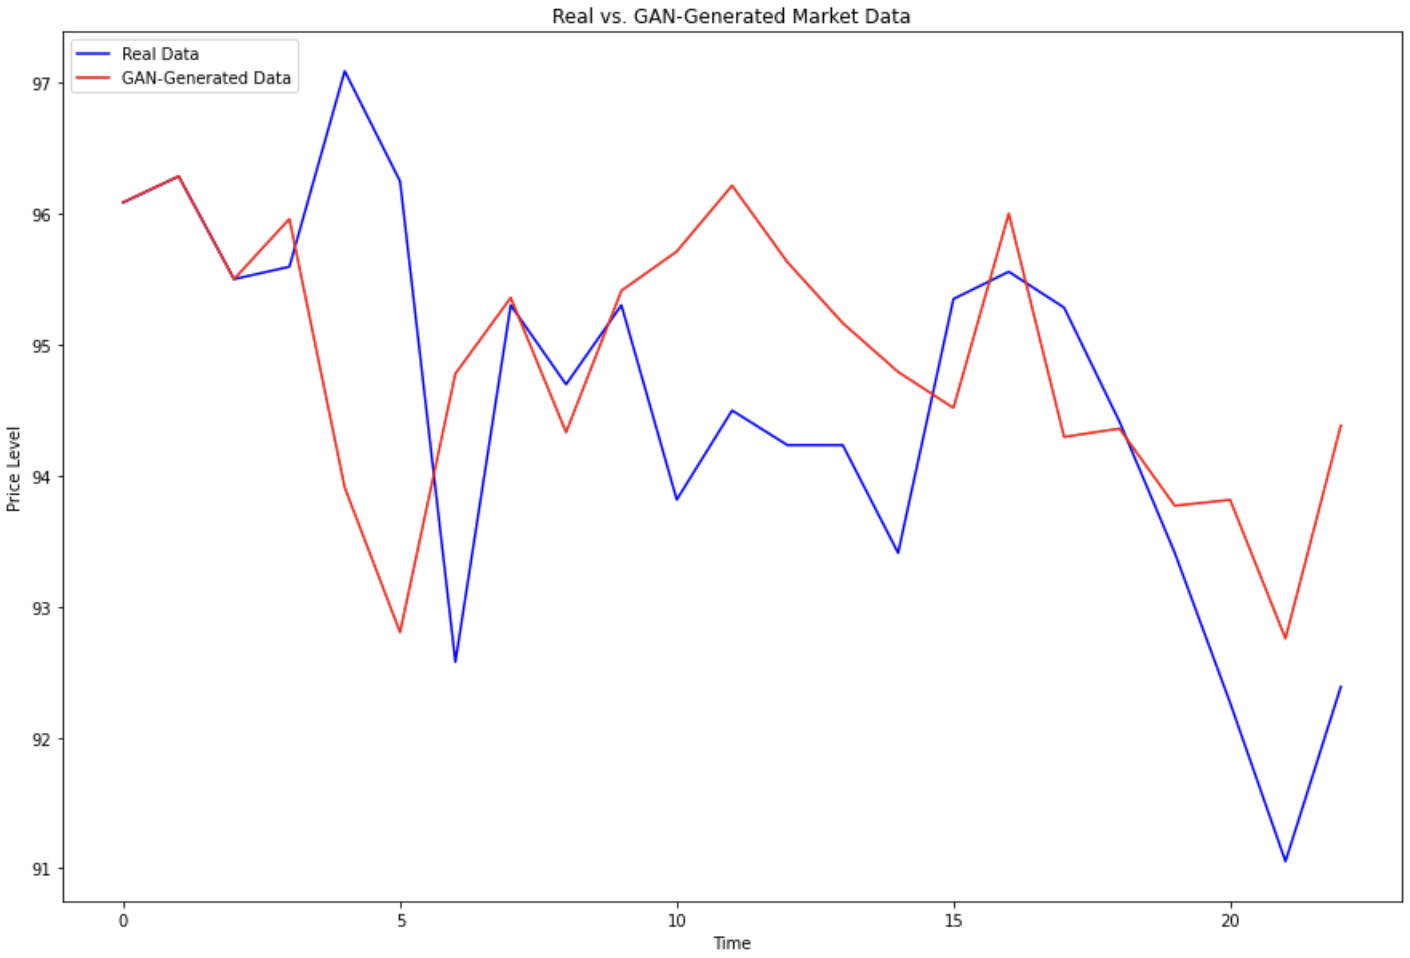
\includegraphics[width=14cm]{templates/assets/gan/gan_stable.png}
\caption{GAN-Based Spot Price Simulation}
\end{figure}

\section{Evaluating GAN-Based Market Simulations}
To be confident in the accuracy of GAN-generated market data in representing empirical data, there must be a systematic framework for evaluating the similarity of synthetic data to real data. However, since GANs are an unsupervised machine learning framework, there isn't a single or standard way to evaluate performance. With supervised machine learning methods, the standard way of measuring performance is to make predictions on a test data set and compute a metric such as accuracy or root mean square error. Since GANs are generating new data, it is infeasible to use the same evaluation methods. However, this does not mean we cannot measure the similarity between GAN-generated synthetic data and real data, but we must be more creative with the evaluation methods.

\subsection{Time-Series Distributional Statistics \& Metrics}

\subsection{t-SNE Comparison}
Another method to evaluate how representative the generator's synthetic data is of empirical data is to use the t-SNE\cite{tsne} algorithm. As high-dimensional data is very difficult to visualize, the t-distributed stochastic neighbor embedding (t-SNE) method visualizes the high-dimensional inputs by mapping the data from a high-dimension to a low-dimension. Using this method, we can compare the t-SNE visualizations between generated data and real data.
